% Options for packages loaded elsewhere
% Options for packages loaded elsewhere
\PassOptionsToPackage{unicode}{hyperref}
\PassOptionsToPackage{hyphens}{url}
\PassOptionsToPackage{dvipsnames,svgnames,x11names}{xcolor}
%
\documentclass[
  spanish,
  letterpaper,
  DIV=11,
  numbers=noendperiod]{scrartcl}
\usepackage{xcolor}
\usepackage{amsmath,amssymb}
\setcounter{secnumdepth}{-\maxdimen} % remove section numbering
\usepackage{iftex}
\ifPDFTeX
  \usepackage[T1]{fontenc}
  \usepackage[utf8]{inputenc}
  \usepackage{textcomp} % provide euro and other symbols
\else % if luatex or xetex
  \usepackage{unicode-math} % this also loads fontspec
  \defaultfontfeatures{Scale=MatchLowercase}
  \defaultfontfeatures[\rmfamily]{Ligatures=TeX,Scale=1}
\fi
\usepackage{lmodern}
\ifPDFTeX\else
  % xetex/luatex font selection
\fi
% Use upquote if available, for straight quotes in verbatim environments
\IfFileExists{upquote.sty}{\usepackage{upquote}}{}
\IfFileExists{microtype.sty}{% use microtype if available
  \usepackage[]{microtype}
  \UseMicrotypeSet[protrusion]{basicmath} % disable protrusion for tt fonts
}{}
\makeatletter
\@ifundefined{KOMAClassName}{% if non-KOMA class
  \IfFileExists{parskip.sty}{%
    \usepackage{parskip}
  }{% else
    \setlength{\parindent}{0pt}
    \setlength{\parskip}{6pt plus 2pt minus 1pt}}
}{% if KOMA class
  \KOMAoptions{parskip=half}}
\makeatother
% Make \paragraph and \subparagraph free-standing
\makeatletter
\ifx\paragraph\undefined\else
  \let\oldparagraph\paragraph
  \renewcommand{\paragraph}{
    \@ifstar
      \xxxParagraphStar
      \xxxParagraphNoStar
  }
  \newcommand{\xxxParagraphStar}[1]{\oldparagraph*{#1}\mbox{}}
  \newcommand{\xxxParagraphNoStar}[1]{\oldparagraph{#1}\mbox{}}
\fi
\ifx\subparagraph\undefined\else
  \let\oldsubparagraph\subparagraph
  \renewcommand{\subparagraph}{
    \@ifstar
      \xxxSubParagraphStar
      \xxxSubParagraphNoStar
  }
  \newcommand{\xxxSubParagraphStar}[1]{\oldsubparagraph*{#1}\mbox{}}
  \newcommand{\xxxSubParagraphNoStar}[1]{\oldsubparagraph{#1}\mbox{}}
\fi
\makeatother

\usepackage{color}
\usepackage{fancyvrb}
\newcommand{\VerbBar}{|}
\newcommand{\VERB}{\Verb[commandchars=\\\{\}]}
\DefineVerbatimEnvironment{Highlighting}{Verbatim}{commandchars=\\\{\}}
% Add ',fontsize=\small' for more characters per line
\usepackage{framed}
\definecolor{shadecolor}{RGB}{241,243,245}
\newenvironment{Shaded}{\begin{snugshade}}{\end{snugshade}}
\newcommand{\AlertTok}[1]{\textcolor[rgb]{0.68,0.00,0.00}{#1}}
\newcommand{\AnnotationTok}[1]{\textcolor[rgb]{0.37,0.37,0.37}{#1}}
\newcommand{\AttributeTok}[1]{\textcolor[rgb]{0.40,0.45,0.13}{#1}}
\newcommand{\BaseNTok}[1]{\textcolor[rgb]{0.68,0.00,0.00}{#1}}
\newcommand{\BuiltInTok}[1]{\textcolor[rgb]{0.00,0.23,0.31}{#1}}
\newcommand{\CharTok}[1]{\textcolor[rgb]{0.13,0.47,0.30}{#1}}
\newcommand{\CommentTok}[1]{\textcolor[rgb]{0.37,0.37,0.37}{#1}}
\newcommand{\CommentVarTok}[1]{\textcolor[rgb]{0.37,0.37,0.37}{\textit{#1}}}
\newcommand{\ConstantTok}[1]{\textcolor[rgb]{0.56,0.35,0.01}{#1}}
\newcommand{\ControlFlowTok}[1]{\textcolor[rgb]{0.00,0.23,0.31}{\textbf{#1}}}
\newcommand{\DataTypeTok}[1]{\textcolor[rgb]{0.68,0.00,0.00}{#1}}
\newcommand{\DecValTok}[1]{\textcolor[rgb]{0.68,0.00,0.00}{#1}}
\newcommand{\DocumentationTok}[1]{\textcolor[rgb]{0.37,0.37,0.37}{\textit{#1}}}
\newcommand{\ErrorTok}[1]{\textcolor[rgb]{0.68,0.00,0.00}{#1}}
\newcommand{\ExtensionTok}[1]{\textcolor[rgb]{0.00,0.23,0.31}{#1}}
\newcommand{\FloatTok}[1]{\textcolor[rgb]{0.68,0.00,0.00}{#1}}
\newcommand{\FunctionTok}[1]{\textcolor[rgb]{0.28,0.35,0.67}{#1}}
\newcommand{\ImportTok}[1]{\textcolor[rgb]{0.00,0.46,0.62}{#1}}
\newcommand{\InformationTok}[1]{\textcolor[rgb]{0.37,0.37,0.37}{#1}}
\newcommand{\KeywordTok}[1]{\textcolor[rgb]{0.00,0.23,0.31}{\textbf{#1}}}
\newcommand{\NormalTok}[1]{\textcolor[rgb]{0.00,0.23,0.31}{#1}}
\newcommand{\OperatorTok}[1]{\textcolor[rgb]{0.37,0.37,0.37}{#1}}
\newcommand{\OtherTok}[1]{\textcolor[rgb]{0.00,0.23,0.31}{#1}}
\newcommand{\PreprocessorTok}[1]{\textcolor[rgb]{0.68,0.00,0.00}{#1}}
\newcommand{\RegionMarkerTok}[1]{\textcolor[rgb]{0.00,0.23,0.31}{#1}}
\newcommand{\SpecialCharTok}[1]{\textcolor[rgb]{0.37,0.37,0.37}{#1}}
\newcommand{\SpecialStringTok}[1]{\textcolor[rgb]{0.13,0.47,0.30}{#1}}
\newcommand{\StringTok}[1]{\textcolor[rgb]{0.13,0.47,0.30}{#1}}
\newcommand{\VariableTok}[1]{\textcolor[rgb]{0.07,0.07,0.07}{#1}}
\newcommand{\VerbatimStringTok}[1]{\textcolor[rgb]{0.13,0.47,0.30}{#1}}
\newcommand{\WarningTok}[1]{\textcolor[rgb]{0.37,0.37,0.37}{\textit{#1}}}

\usepackage{longtable,booktabs,array}
\newcounter{none} % for unnumbered tables
\usepackage{calc} % for calculating minipage widths
% Correct order of tables after \paragraph or \subparagraph
\usepackage{etoolbox}
\makeatletter
\patchcmd\longtable{\par}{\if@noskipsec\mbox{}\fi\par}{}{}
\makeatother
% Allow footnotes in longtable head/foot
\IfFileExists{footnotehyper.sty}{\usepackage{footnotehyper}}{\usepackage{footnote}}
\makesavenoteenv{longtable}
\usepackage{graphicx}
\makeatletter
\newsavebox\pandoc@box
\newcommand*\pandocbounded[1]{% scales image to fit in text height/width
  \sbox\pandoc@box{#1}%
  \Gscale@div\@tempa{\textheight}{\dimexpr\ht\pandoc@box+\dp\pandoc@box\relax}%
  \Gscale@div\@tempb{\linewidth}{\wd\pandoc@box}%
  \ifdim\@tempb\p@<\@tempa\p@\let\@tempa\@tempb\fi% select the smaller of both
  \ifdim\@tempa\p@<\p@\scalebox{\@tempa}{\usebox\pandoc@box}%
  \else\usebox{\pandoc@box}%
  \fi%
}
% Set default figure placement to htbp
\def\fps@figure{htbp}
\makeatother


% definitions for citeproc citations
\NewDocumentCommand\citeproctext{}{}
\NewDocumentCommand\citeproc{mm}{%
  \begingroup\def\citeproctext{#2}\cite{#1}\endgroup}
\makeatletter
 % allow citations to break across lines
 \let\@cite@ofmt\@firstofone
 % avoid brackets around text for \cite:
 \def\@biblabel#1{}
 \def\@cite#1#2{{#1\if@tempswa , #2\fi}}
\makeatother
\newlength{\cslhangindent}
\setlength{\cslhangindent}{1.5em}
\newlength{\csllabelwidth}
\setlength{\csllabelwidth}{3em}
\newenvironment{CSLReferences}[2] % #1 hanging-indent, #2 entry-spacing
 {\begin{list}{}{%
  \setlength{\itemindent}{0pt}
  \setlength{\leftmargin}{0pt}
  \setlength{\parsep}{0pt}
  % turn on hanging indent if param 1 is 1
  \ifodd #1
   \setlength{\leftmargin}{\cslhangindent}
   \setlength{\itemindent}{-1\cslhangindent}
  \fi
  % set entry spacing
  \setlength{\itemsep}{#2\baselineskip}}}
 {\end{list}}
\usepackage{calc}
\newcommand{\CSLBlock}[1]{\hfill\break\parbox[t]{\linewidth}{\strut\ignorespaces#1\strut}}
\newcommand{\CSLLeftMargin}[1]{\parbox[t]{\csllabelwidth}{\strut#1\strut}}
\newcommand{\CSLRightInline}[1]{\parbox[t]{\linewidth - \csllabelwidth}{\strut#1\strut}}
\newcommand{\CSLIndent}[1]{\hspace{\cslhangindent}#1}

\ifLuaTeX
\usepackage[bidi=basic,shorthands=off]{babel}
\else
\usepackage[bidi=default,shorthands=off]{babel}
\fi
\ifLuaTeX
  \usepackage{selnolig} % disable illegal ligatures
\fi


\setlength{\emergencystretch}{3em} % prevent overfull lines

\providecommand{\tightlist}{%
  \setlength{\itemsep}{0pt}\setlength{\parskip}{0pt}}



 


\KOMAoption{captions}{tableheading}
\makeatletter
\@ifpackageloaded{caption}{}{\usepackage{caption}}
\AtBeginDocument{%
\ifdefined\contentsname
  \renewcommand*\contentsname{Tabla de contenidos}
\else
  \newcommand\contentsname{Tabla de contenidos}
\fi
\ifdefined\listfigurename
  \renewcommand*\listfigurename{Listado de Figuras}
\else
  \newcommand\listfigurename{Listado de Figuras}
\fi
\ifdefined\listtablename
  \renewcommand*\listtablename{Listado de Tablas}
\else
  \newcommand\listtablename{Listado de Tablas}
\fi
\ifdefined\figurename
  \renewcommand*\figurename{Figura}
\else
  \newcommand\figurename{Figura}
\fi
\ifdefined\tablename
  \renewcommand*\tablename{Tabla}
\else
  \newcommand\tablename{Tabla}
\fi
}
\@ifpackageloaded{float}{}{\usepackage{float}}
\floatstyle{ruled}
\@ifundefined{c@chapter}{\newfloat{codelisting}{h}{lop}}{\newfloat{codelisting}{h}{lop}[chapter]}
\floatname{codelisting}{Listado}
\newcommand*\listoflistings{\listof{codelisting}{Listado de Listados}}
\makeatother
\makeatletter
\makeatother
\makeatletter
\@ifpackageloaded{caption}{}{\usepackage{caption}}
\@ifpackageloaded{subcaption}{}{\usepackage{subcaption}}
\makeatother
\usepackage{bookmark}
\IfFileExists{xurl.sty}{\usepackage{xurl}}{} % add URL line breaks if available
\urlstyle{same}
% fallback for those not using the hyperref driver hyperxmp:
\makeatletter
\@ifundefined{xmpquote}{\newcommand{\xmpquote}[1]{#1}}{}
\makeatother
\hypersetup{
  pdflang={es},
  colorlinks=true,
  linkcolor={blue},
  filecolor={Maroon},
  citecolor={Blue},
  urlcolor={Blue},
  pdfcreator={LaTeX via pandoc}}


\author{}
\date{}
\begin{document}


\pandocbounded{
\includegraphics[keepaspectratio]{resources/banner.jpg}}

\section{Recopilación de datos}\label{recopilaciuxf3n-de-datos}

\subsection{Marco Geoestádistico del
INEGI}\label{marco-geoestuxe1distico-del-inegi}

Usamos las capas de AGEB (Área Geoestadística Básica) urbana y rural, y
localidad amanzanada de
\href{https://www.inegi.org.mx/programas/mg/\#mapas}{la página del
INEGI}, a escala Ciudad de México.

De acuerdo al glosario del INEGI (\citeproc{ref-inegiGlosario}{s.~f.})

\begin{quote}
\textbf{Área geoestadística básica (AGEB)}:

Subdivisión de los municipios o delegaciones que conforman el país,
utilizada por vez primera en el X Censo General de Población y Vivienda
1980, que permite la formación de unidades primarias de muestreo y la
organización de la información estadística. Tiene tres atributos
fundamentales: a) es perfectamente reconocible en el terreno, por estar
delimitada por rasgos topográficos identificables y perdurables; b)
generalmente es homogénea en cuanto a sus características geográficas,
económicas y sociales; c) su extensión es tal que puede ser recorrida
por una sola persona. Las AGEB se clasifican en más urbanizadas y menos
urbanizadas. Una AGEB más urbanizada puede variar de tamaño entre 20 y
80 manzanas, mientras que una AGEB menos urbanizada puede comprender una
o más localidades menores a 100 000 habitantes, dependiendo en ambos
casos de la densidad de viviendas.
\end{quote}

Las capas se descargan por separado, y fueron renombradas para coincidir
con la capa que representan.

\begin{Shaded}
\begin{Highlighting}[]
\ImportTok{import}\NormalTok{ geopandas }\ImportTok{as}\NormalTok{ gpd}
\ImportTok{import}\NormalTok{ matplotlib.patches }\ImportTok{as}\NormalTok{ mpatches}
\ImportTok{import}\NormalTok{ matplotlib.pyplot }\ImportTok{as}\NormalTok{ plt}

\CommentTok{\# 1. Cargar capas de INEGI}
\NormalTok{MUNICIPIOS }\OperatorTok{=}\NormalTok{ [}\StringTok{\textquotesingle{}009\textquotesingle{}}\NormalTok{, }\StringTok{\textquotesingle{}011\textquotesingle{}}\NormalTok{, }\StringTok{\textquotesingle{}013\textquotesingle{}}\NormalTok{]}
\NormalTok{NOMBRES\_MUN }\OperatorTok{=}\NormalTok{ \{}\StringTok{\textquotesingle{}009\textquotesingle{}}\NormalTok{: }\StringTok{\textquotesingle{}Milpa Alta\textquotesingle{}}\NormalTok{, }\StringTok{\textquotesingle{}011\textquotesingle{}}\NormalTok{: }\StringTok{\textquotesingle{}Tláhuac\textquotesingle{}}\NormalTok{, }\StringTok{\textquotesingle{}013\textquotesingle{}}\NormalTok{: }\StringTok{\textquotesingle{}Xochimilco\textquotesingle{}}\NormalTok{\}}

\NormalTok{ageb\_urb }\OperatorTok{=}\NormalTok{ gpd.read\_file(}\StringTok{"../data/ageb\_urbano/ageb\_urbano.shp"}\NormalTok{)}
\NormalTok{ageb\_rur }\OperatorTok{=}\NormalTok{ gpd.read\_file(}\StringTok{"../data/ageb\_rural/ageb\_rural.shp"}\NormalTok{)}

\CommentTok{\# 2. Filtrar las 3 alcaldías y proyectar a Web Mercator (EPSG:3857)}
\NormalTok{urb\_sur }\OperatorTok{=}\NormalTok{ ageb\_urb[ageb\_urb[}\StringTok{\textquotesingle{}CVE\_MUN\textquotesingle{}}\NormalTok{].isin(MUNICIPIOS)].to\_crs(epsg}\OperatorTok{=}\DecValTok{3857}\NormalTok{).copy()}
\NormalTok{rur\_sur }\OperatorTok{=}\NormalTok{ ageb\_rur[ageb\_rur[}\StringTok{\textquotesingle{}CVE\_MUN\textquotesingle{}}\NormalTok{].isin(MUNICIPIOS)].to\_crs(epsg}\OperatorTok{=}\DecValTok{3857}\NormalTok{).copy()}

\CommentTok{\# 3. Asignar etiquetas legibles de alcaldía y tipo}
\NormalTok{urb\_sur[}\StringTok{\textquotesingle{}Alcaldia\textquotesingle{}}\NormalTok{] }\OperatorTok{=}\NormalTok{ urb\_sur[}\StringTok{\textquotesingle{}CVE\_MUN\textquotesingle{}}\NormalTok{].}\BuiltInTok{map}\NormalTok{(NOMBRES\_MUN)}
\NormalTok{urb\_sur[}\StringTok{\textquotesingle{}Tipo\textquotesingle{}}\NormalTok{] }\OperatorTok{=} \StringTok{\textquotesingle{}Urbano\textquotesingle{}}
\NormalTok{urb\_sur[}\StringTok{\textquotesingle{}Categoria\textquotesingle{}}\NormalTok{] }\OperatorTok{=}\NormalTok{ urb\_sur[}\StringTok{\textquotesingle{}Alcaldia\textquotesingle{}}\NormalTok{] }\OperatorTok{+} \StringTok{" {-} Urbano"}

\NormalTok{rur\_sur[}\StringTok{\textquotesingle{}Alcaldia\textquotesingle{}}\NormalTok{] }\OperatorTok{=}\NormalTok{ rur\_sur[}\StringTok{\textquotesingle{}CVE\_MUN\textquotesingle{}}\NormalTok{].}\BuiltInTok{map}\NormalTok{(NOMBRES\_MUN)}
\NormalTok{rur\_sur[}\StringTok{\textquotesingle{}Tipo\textquotesingle{}}\NormalTok{] }\OperatorTok{=} \StringTok{\textquotesingle{}Rural\textquotesingle{}}
\NormalTok{rur\_sur[}\StringTok{\textquotesingle{}Categoria\textquotesingle{}}\NormalTok{] }\OperatorTok{=}\NormalTok{ rur\_sur[}\StringTok{\textquotesingle{}Alcaldia\textquotesingle{}}\NormalTok{] }\OperatorTok{+} \StringTok{" {-} Rural"}

\CommentTok{\# 4. Definición de paleta (Color de relleno, color de borde)}
\CommentTok{\# Se eligen tonos contrastantes pero coherentes por zona}
\NormalTok{ESTILOS }\OperatorTok{=}\NormalTok{ \{}
    \StringTok{\textquotesingle{}Xochimilco {-} Urbano\textquotesingle{}}\NormalTok{:   \{}\StringTok{\textquotesingle{}fill\textquotesingle{}}\NormalTok{: }\StringTok{\textquotesingle{}\#e41a1c\textquotesingle{}}\NormalTok{, }\StringTok{\textquotesingle{}edge\textquotesingle{}}\NormalTok{: }\StringTok{\textquotesingle{}\#7f0000\textquotesingle{}}\NormalTok{, }\StringTok{\textquotesingle{}alpha\textquotesingle{}}\NormalTok{: }\FloatTok{0.65}\NormalTok{\},  }\CommentTok{\# Rojo intenso}
    \StringTok{\textquotesingle{}Xochimilco {-} Rural\textquotesingle{}}\NormalTok{:    \{}\StringTok{\textquotesingle{}fill\textquotesingle{}}\NormalTok{: }\StringTok{\textquotesingle{}\#fc9272\textquotesingle{}}\NormalTok{, }\StringTok{\textquotesingle{}edge\textquotesingle{}}\NormalTok{: }\StringTok{\textquotesingle{}\#de2d26\textquotesingle{}}\NormalTok{, }\StringTok{\textquotesingle{}alpha\textquotesingle{}}\NormalTok{: }\FloatTok{0.45}\NormalTok{\},  }\CommentTok{\# Salmón / terracota}
    \StringTok{\textquotesingle{}Tláhuac {-} Urbano\textquotesingle{}}\NormalTok{:       \{}\StringTok{\textquotesingle{}fill\textquotesingle{}}\NormalTok{: }\StringTok{\textquotesingle{}\#1f78b4\textquotesingle{}}\NormalTok{, }\StringTok{\textquotesingle{}edge\textquotesingle{}}\NormalTok{: }\StringTok{\textquotesingle{}\#084594\textquotesingle{}}\NormalTok{, }\StringTok{\textquotesingle{}alpha\textquotesingle{}}\NormalTok{: }\FloatTok{0.65}\NormalTok{\},  }\CommentTok{\# Azul cobalto}
    \StringTok{\textquotesingle{}Tláhuac {-} Rural\textquotesingle{}}\NormalTok{:        \{}\StringTok{\textquotesingle{}fill\textquotesingle{}}\NormalTok{: }\StringTok{\textquotesingle{}\#a6cee3\textquotesingle{}}\NormalTok{, }\StringTok{\textquotesingle{}edge\textquotesingle{}}\NormalTok{: }\StringTok{\textquotesingle{}\#2171b5\textquotesingle{}}\NormalTok{, }\StringTok{\textquotesingle{}alpha\textquotesingle{}}\NormalTok{: }\FloatTok{0.45}\NormalTok{\},  }\CommentTok{\# Azul cielo}
    \StringTok{\textquotesingle{}Milpa Alta {-} Urbano\textquotesingle{}}\NormalTok{:    \{}\StringTok{\textquotesingle{}fill\textquotesingle{}}\NormalTok{: }\StringTok{\textquotesingle{}\#33a02c\textquotesingle{}}\NormalTok{, }\StringTok{\textquotesingle{}edge\textquotesingle{}}\NormalTok{: }\StringTok{\textquotesingle{}\#00441b\textquotesingle{}}\NormalTok{, }\StringTok{\textquotesingle{}alpha\textquotesingle{}}\NormalTok{: }\FloatTok{0.65}\NormalTok{\},  }\CommentTok{\# Verde bosque}
    \StringTok{\textquotesingle{}Milpa Alta {-} Rural\textquotesingle{}}\NormalTok{:     \{}\StringTok{\textquotesingle{}fill\textquotesingle{}}\NormalTok{: }\StringTok{\textquotesingle{}\#b2df8a\textquotesingle{}}\NormalTok{, }\StringTok{\textquotesingle{}edge\textquotesingle{}}\NormalTok{: }\StringTok{\textquotesingle{}\#238b45\textquotesingle{}}\NormalTok{, }\StringTok{\textquotesingle{}alpha\textquotesingle{}}\NormalTok{: }\FloatTok{0.40}\NormalTok{\},  }\CommentTok{\# Verde pasto}
\NormalTok{\}}

\CommentTok{\# 5. Graficar}
\NormalTok{fig, ax }\OperatorTok{=}\NormalTok{ plt.subplots(figsize}\OperatorTok{=}\NormalTok{(}\DecValTok{13}\NormalTok{, }\DecValTok{12}\NormalTok{))}

\CommentTok{\# Pintar capas rurales primero (fondo) y luego urbanas (frente)}
\ControlFlowTok{for}\NormalTok{ cat, estilo }\KeywordTok{in}\NormalTok{ ESTILOS.items():}
    \ControlFlowTok{if} \StringTok{"Rural"} \KeywordTok{in}\NormalTok{ cat:}
\NormalTok{        sub\_gdf }\OperatorTok{=}\NormalTok{ rur\_sur[rur\_sur[}\StringTok{\textquotesingle{}Categoria\textquotesingle{}}\NormalTok{] }\OperatorTok{==}\NormalTok{ cat]}
\NormalTok{        sub\_gdf.plot(}
\NormalTok{            ax}\OperatorTok{=}\NormalTok{ax,}
\NormalTok{            facecolor}\OperatorTok{=}\NormalTok{estilo[}\StringTok{\textquotesingle{}fill\textquotesingle{}}\NormalTok{],}
\NormalTok{            edgecolor}\OperatorTok{=}\NormalTok{estilo[}\StringTok{\textquotesingle{}edge\textquotesingle{}}\NormalTok{],}
\NormalTok{            linewidth}\OperatorTok{=}\FloatTok{0.7}\NormalTok{,}
\NormalTok{            alpha}\OperatorTok{=}\NormalTok{estilo[}\StringTok{\textquotesingle{}alpha\textquotesingle{}}\NormalTok{]}
\NormalTok{        )}
    \ControlFlowTok{elif} \StringTok{"Urbano"} \KeywordTok{in}\NormalTok{ cat:}
\NormalTok{        sub\_gdf }\OperatorTok{=}\NormalTok{ urb\_sur[urb\_sur[}\StringTok{\textquotesingle{}Categoria\textquotesingle{}}\NormalTok{] }\OperatorTok{==}\NormalTok{ cat]}
\NormalTok{        sub\_gdf.plot(}
\NormalTok{            ax}\OperatorTok{=}\NormalTok{ax,}
\NormalTok{            facecolor}\OperatorTok{=}\NormalTok{estilo[}\StringTok{\textquotesingle{}fill\textquotesingle{}}\NormalTok{],}
\NormalTok{            edgecolor}\OperatorTok{=}\NormalTok{estilo[}\StringTok{\textquotesingle{}edge\textquotesingle{}}\NormalTok{],}
\NormalTok{            linewidth}\OperatorTok{=}\FloatTok{0.5}\NormalTok{,}
\NormalTok{            alpha}\OperatorTok{=}\NormalTok{estilo[}\StringTok{\textquotesingle{}alpha\textquotesingle{}}\NormalTok{]}
\NormalTok{        )}

\CommentTok{\# 6. Añadir mapa base satelital}
\ControlFlowTok{try}\NormalTok{:}
    \ImportTok{import}\NormalTok{ contextily }\ImportTok{as}\NormalTok{ ctx}
\NormalTok{    ctx.add\_basemap(ax, source}\OperatorTok{=}\StringTok{"Esri.WorldImagery"}\NormalTok{)}
\ControlFlowTok{except} \PreprocessorTok{Exception} \ImportTok{as}\NormalTok{ e:}
    \BuiltInTok{print}\NormalTok{(}\SpecialStringTok{f"Aviso mapa base: }\SpecialCharTok{\{}\NormalTok{e}\SpecialCharTok{\}}\SpecialStringTok{"}\NormalTok{)}

\CommentTok{\# 7. Construir leyenda personalizada}
\NormalTok{parches\_leyenda }\OperatorTok{=}\NormalTok{ [}
\NormalTok{    mpatches.Patch(}
\NormalTok{        facecolor}\OperatorTok{=}\NormalTok{estilo[}\StringTok{\textquotesingle{}fill\textquotesingle{}}\NormalTok{],}
\NormalTok{        edgecolor}\OperatorTok{=}\NormalTok{estilo[}\StringTok{\textquotesingle{}edge\textquotesingle{}}\NormalTok{],}
\NormalTok{        label}\OperatorTok{=}\NormalTok{cat,}
\NormalTok{        alpha}\OperatorTok{=}\NormalTok{estilo[}\StringTok{\textquotesingle{}alpha\textquotesingle{}}\NormalTok{]}
\NormalTok{    )}
    \ControlFlowTok{for}\NormalTok{ cat, estilo }\KeywordTok{in}\NormalTok{ ESTILOS.items()}
\NormalTok{]}

\NormalTok{ax.legend(}
\NormalTok{    handles}\OperatorTok{=}\NormalTok{parches\_leyenda,}
\NormalTok{    title}\OperatorTok{=}\StringTok{"Alcaldía y Ámbito"}\NormalTok{,}
\NormalTok{    loc}\OperatorTok{=}\StringTok{"lower left"}\NormalTok{,}
\NormalTok{    frameon}\OperatorTok{=}\VariableTok{True}\NormalTok{,}
\NormalTok{    facecolor}\OperatorTok{=}\StringTok{"white"}\NormalTok{,}
\NormalTok{    framealpha}\OperatorTok{=}\FloatTok{0.9}\NormalTok{,}
\NormalTok{    fontsize}\OperatorTok{=}\DecValTok{9}\NormalTok{,}
\NormalTok{    title\_fontsize}\OperatorTok{=}\DecValTok{10}
\NormalTok{)}

\NormalTok{ax.set\_title(}
    \StringTok{"Área Urbana vs. Rural por Alcaldía (INEGI Marco Geoestadístico)}\CharTok{\textbackslash{}n}\StringTok{Xochimilco, Tláhuac y Milpa Alta"}\NormalTok{,}
\NormalTok{    fontsize}\OperatorTok{=}\DecValTok{13}\NormalTok{,}
\NormalTok{    pad}\OperatorTok{=}\DecValTok{12}
\NormalTok{)}
\NormalTok{ax.set\_axis\_off()}
\NormalTok{plt.tight\_layout()}
\NormalTok{plt.show()}
\end{Highlighting}
\end{Shaded}

\pandocbounded{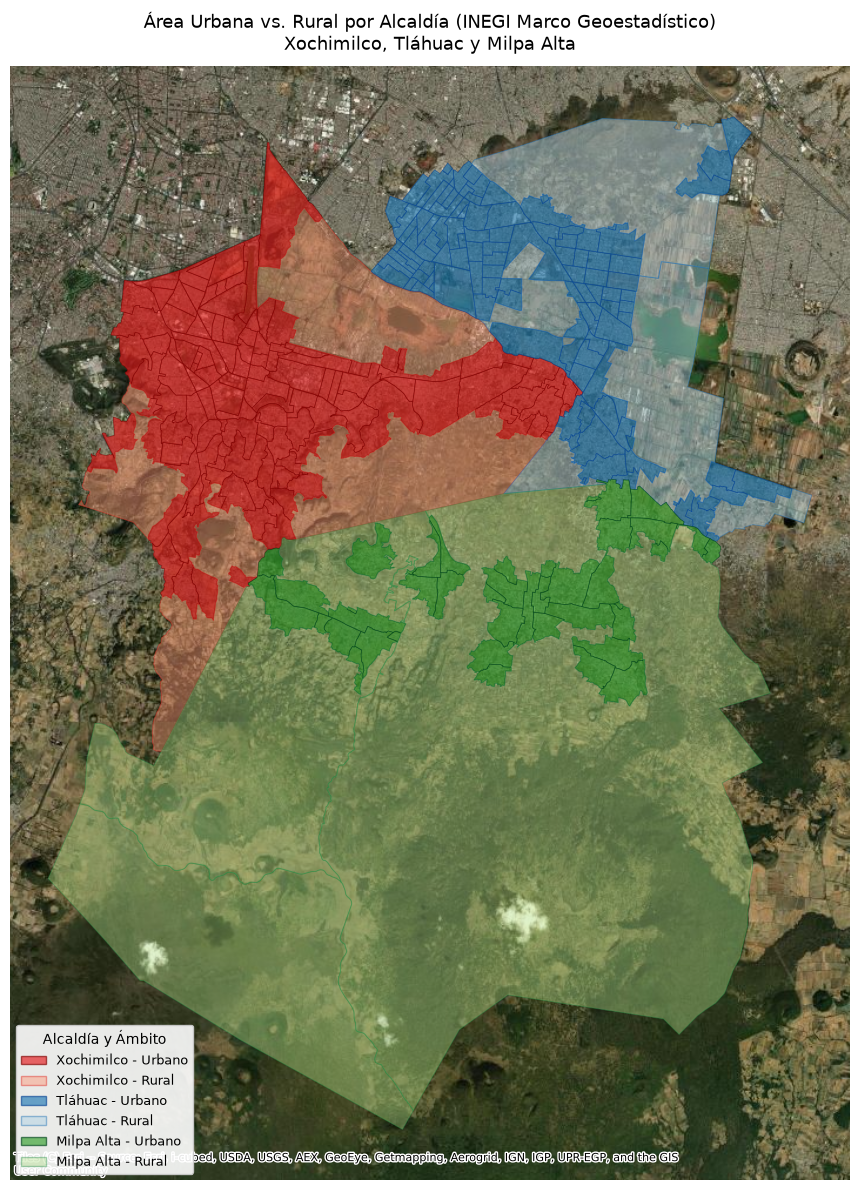
\includegraphics[keepaspectratio]{exploracion_files/figure-pdf/cell-2-output-1.png}}

\subsection{Catálogo de Colonias de la Ciudad de México (Datos Abiertos
CDMX)}\label{catuxe1logo-de-colonias-de-la-ciudad-de-muxe9xico-datos-abiertos-cdmx}

Es la delimitación geográfica oficial de las unidades territoriales,
colonias, barrios y pueblos originarios reconocidos por la
administración pública de la Ciudad de México.

Mantenida por: Agencia Digital de Innovación Pública (ADIP) / Secretaría
de Desarrollo Urbano y Vivienda (SEDUVI).

A diferencia del Marco Geoestadístico de INEGI (que segmenta en AGEBs
numéricas arbitrarias por densidad poblacional para fines censales),
esta capa conserva los nombres y las delimitaciones comunitarias,
permitiendo acotar a Santiago Tulyehualco y las colonias que lo
integran.

Disponible en la
\href{https://datos.cdmx.gob.mx/dataset/catalogo-de-colonias-datos-abiertos}{página
de datos abiertos de la CDMX}.

\begin{Shaded}
\begin{Highlighting}[]
\ImportTok{import}\NormalTok{ geopandas }\ImportTok{as}\NormalTok{ gpd}

\NormalTok{colonias\_cdmx }\OperatorTok{=}\NormalTok{ gpd.read\_file(}\StringTok{"../data/mapa\_colonias.json"}\NormalTok{)}
\BuiltInTok{print}\NormalTok{(colonias\_cdmx.crs)}

\CommentTok{\# Si no tiene CRS definido en el JSON, se lo asignamos primero como EPSG:4326}
\ControlFlowTok{if}\NormalTok{ colonias\_cdmx.crs }\KeywordTok{is} \VariableTok{None}\NormalTok{:}
\NormalTok{    colonias\_cdmx }\OperatorTok{=}\NormalTok{ colonias\_cdmx.set\_crs(epsg}\OperatorTok{=}\DecValTok{4326}\NormalTok{)}

\CommentTok{\# Ahora sí lo proyectamos a Web Mercator para contextily}
\NormalTok{colonias\_cdmx }\OperatorTok{=}\NormalTok{ colonias\_cdmx.to\_crs(epsg}\OperatorTok{=}\DecValTok{3857}\NormalTok{)}


\NormalTok{cols\_nombre\_colonia }\OperatorTok{=} \StringTok{"colonia"}
\NormalTok{cols\_nombre\_alcaldia }\OperatorTok{=} \StringTok{"alc"}

\NormalTok{CLAVES\_SUR }\OperatorTok{=}\NormalTok{ [}\StringTok{"009"}\NormalTok{, }\StringTok{"011"}\NormalTok{, }\StringTok{"013"}\NormalTok{, }\StringTok{"9"}\NormalTok{, }\StringTok{"11"}\NormalTok{, }\StringTok{"13"}\NormalTok{, }\StringTok{"09"}\NormalTok{, }\StringTok{"11"}\NormalTok{, }\StringTok{"13"}\NormalTok{]}


\NormalTok{filtro\_sur }\OperatorTok{=}\NormalTok{ colonias\_cdmx[cols\_nombre\_alcaldia].astype(}\BuiltInTok{str}\NormalTok{).}\BuiltInTok{str}\NormalTok{.upper().}\BuiltInTok{str}\NormalTok{.contains(}
    \StringTok{"XOCHIMILCO|TL[AÁ]HUAC|MILPA ALTA"}\NormalTok{, regex}\OperatorTok{=}\VariableTok{True}
\NormalTok{)}

\NormalTok{colonias\_sur }\OperatorTok{=}\NormalTok{ colonias\_cdmx[filtro\_sur].copy()}
\BuiltInTok{print}\NormalTok{(}\SpecialStringTok{f"Total de polígonos cargados: }\SpecialCharTok{\{}\BuiltInTok{len}\NormalTok{(colonias\_cdmx)}\SpecialCharTok{\}}\SpecialStringTok{"}\NormalTok{)}
\BuiltInTok{print}\NormalTok{(}\SpecialStringTok{f"Unidades territoriales en el suroriente encontradas: }\SpecialCharTok{\{}\BuiltInTok{len}\NormalTok{(colonias\_sur)}\SpecialCharTok{\}}\SpecialStringTok{"}\NormalTok{)}
\end{Highlighting}
\end{Shaded}

\begin{verbatim}
EPSG:4326
Total de polígonos cargados: 1543
Unidades territoriales en el suroriente encontradas: 232
\end{verbatim}

\begin{Shaded}
\begin{Highlighting}[]
\ImportTok{import}\NormalTok{ matplotlib.pyplot }\ImportTok{as}\NormalTok{ plt}

\NormalTok{fig, ax }\OperatorTok{=}\NormalTok{ plt.subplots(figsize}\OperatorTok{=}\NormalTok{(}\DecValTok{11}\NormalTok{, }\DecValTok{10}\NormalTok{))}

\NormalTok{colonias\_sur.plot(}
\NormalTok{    column}\OperatorTok{=}\NormalTok{cols\_nombre\_alcaldia,}
\NormalTok{    ax}\OperatorTok{=}\NormalTok{ax,}
\NormalTok{    cmap}\OperatorTok{=}\StringTok{"Set2"}\NormalTok{,}
\NormalTok{    alpha}\OperatorTok{=}\FloatTok{0.55}\NormalTok{,}
\NormalTok{    edgecolor}\OperatorTok{=}\StringTok{"black"}\NormalTok{,}
\NormalTok{    linewidth}\OperatorTok{=}\FloatTok{0.5}\NormalTok{,}
\NormalTok{    legend}\OperatorTok{=}\VariableTok{True}\NormalTok{,}
\NormalTok{    legend\_kwds}\OperatorTok{=}\NormalTok{\{}\StringTok{"title"}\NormalTok{: }\StringTok{"Alcaldía"}\NormalTok{, }\StringTok{"loc"}\NormalTok{: }\StringTok{"lower left"}\NormalTok{, }\StringTok{"frameon"}\NormalTok{: }\VariableTok{True}\NormalTok{\},}
\NormalTok{)}

\ControlFlowTok{try}\NormalTok{:}
    \ImportTok{import}\NormalTok{ contextily }\ImportTok{as}\NormalTok{ ctx}
\NormalTok{    ctx.add\_basemap(ax, source}\OperatorTok{=}\StringTok{"Esri.WorldImagery"}\NormalTok{)}
\ControlFlowTok{except} \PreprocessorTok{Exception} \ImportTok{as}\NormalTok{ e:}
    \BuiltInTok{print}\NormalTok{(}\SpecialStringTok{f"Aviso mapa base: }\SpecialCharTok{\{}\NormalTok{e}\SpecialCharTok{\}}\SpecialStringTok{"}\NormalTok{)}

\NormalTok{ax.set\_title(}
    \StringTok{"Catálogo de Colonias y Pueblos CDMX (Xochimilco, Tláhuac, Milpa Alta) ADIP"}\NormalTok{,}
\NormalTok{    fontsize}\OperatorTok{=}\DecValTok{13}\NormalTok{,}
\NormalTok{    pad}\OperatorTok{=}\DecValTok{12}\NormalTok{,}
\NormalTok{)}
\NormalTok{ax.set\_axis\_off()}
\NormalTok{plt.tight\_layout()}
\NormalTok{plt.show()}
\end{Highlighting}
\end{Shaded}

\pandocbounded{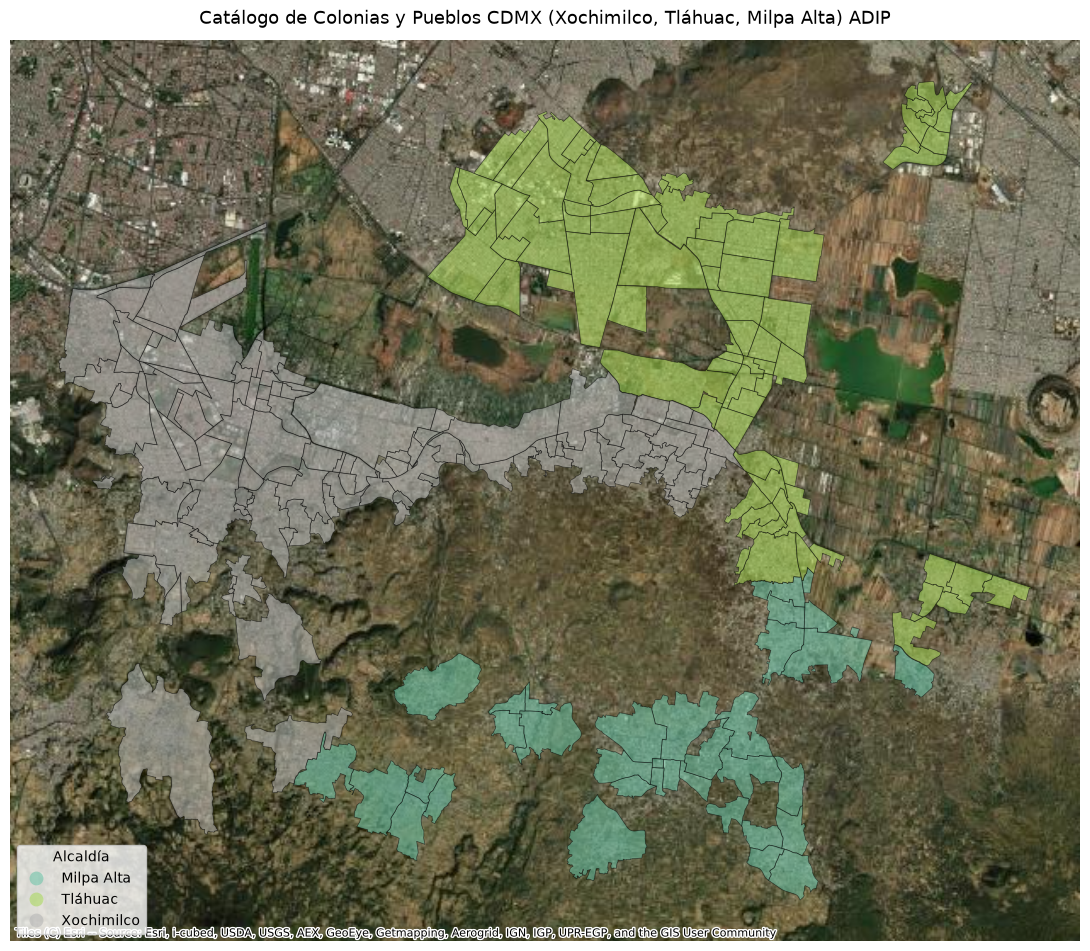
\includegraphics[keepaspectratio]{exploracion_files/figure-pdf/cell-4-output-1.png}}

\subsection{Colonias Electorales: IECM
2019}\label{colonias-electorales-iecm-2019}

Delimitación territorial de las colonias de la Ciudad de México por el
Instituto Electoral de la ciudad de México, versión 2019.

Sirve para contrastar las zonas urbanas de nuestro interés respecto a la
división del INEGI.

Disponible en la
\href{https://datos.cdmx.gob.mx/dataset/coloniascdmx}{plataforma de
datos abiertos de la CDMX}.

\begin{Shaded}
\begin{Highlighting}[]
\ImportTok{import}\NormalTok{ geopandas }\ImportTok{as}\NormalTok{ gpd}
\ImportTok{from}\NormalTok{ IPython.display }\ImportTok{import}\NormalTok{ HTML}

\NormalTok{colonias\_cdmx\_iecm }\OperatorTok{=}\NormalTok{ gpd.read\_file(}\StringTok{"../data/iecm\_2019.json"}\NormalTok{)}

\CommentTok{\# Si no tiene CRS definido en el JSON, se lo asignamos primero como EPSG:4326}
\ControlFlowTok{if}\NormalTok{ colonias\_cdmx\_iecm.crs }\KeywordTok{is} \VariableTok{None}\NormalTok{:}
\NormalTok{    colonias\_cdmx\_iecm }\OperatorTok{=}\NormalTok{ colonias\_cdmx\_iecm.set\_crs(epsg}\OperatorTok{=}\DecValTok{4326}\NormalTok{)}

\CommentTok{\# Ahora sí lo proyectamos a Web Mercator para contextily}
\NormalTok{colonias\_cdmx\_iecm }\OperatorTok{=}\NormalTok{ colonias\_cdmx\_iecm.to\_crs(epsg}\OperatorTok{=}\DecValTok{3857}\NormalTok{)}

\NormalTok{cols\_nombre\_colonia }\OperatorTok{=} \StringTok{"NOMUT"}
\NormalTok{cols\_nombre\_alcaldia }\OperatorTok{=} \StringTok{"NOMDT"}

\NormalTok{CLAVES\_SUR }\OperatorTok{=}\NormalTok{ [}\StringTok{"009"}\NormalTok{, }\StringTok{"011"}\NormalTok{, }\StringTok{"013"}\NormalTok{, }\StringTok{"9"}\NormalTok{, }\StringTok{"11"}\NormalTok{, }\StringTok{"13"}\NormalTok{, }\StringTok{"09"}\NormalTok{, }\StringTok{"11"}\NormalTok{, }\StringTok{"13"}\NormalTok{]}


\NormalTok{filtro\_sur\_iecm }\OperatorTok{=}\NormalTok{ colonias\_cdmx\_iecm[cols\_nombre\_alcaldia].astype(}\BuiltInTok{str}\NormalTok{).}\BuiltInTok{str}\NormalTok{.upper().}\BuiltInTok{str}\NormalTok{.contains(}
    \StringTok{"XOCHIMILCO|TL[AÁ]HUAC|MILPA ALTA"}\NormalTok{, regex}\OperatorTok{=}\VariableTok{True}
\NormalTok{)}

\NormalTok{colonias\_sur\_iecm }\OperatorTok{=}\NormalTok{ colonias\_cdmx\_iecm[filtro\_sur\_iecm].copy()}
\BuiltInTok{print}\NormalTok{(}\SpecialStringTok{f"Total de polígonos cargados: }\SpecialCharTok{\{}\BuiltInTok{len}\NormalTok{(colonias\_cdmx\_iecm)}\SpecialCharTok{\}}\SpecialStringTok{"}\NormalTok{)}
\BuiltInTok{print}\NormalTok{(}\SpecialStringTok{f"Unidades territoriales en el suroriente encontradas: }\SpecialCharTok{\{}\BuiltInTok{len}\NormalTok{(colonias\_sur\_iecm)}\SpecialCharTok{\}}\SpecialStringTok{"}\NormalTok{)}
\end{Highlighting}
\end{Shaded}

\begin{verbatim}
Total de polígonos cargados: 1814
Unidades territoriales en el suroriente encontradas: 150
\end{verbatim}

\begin{Shaded}
\begin{Highlighting}[]
\ImportTok{import}\NormalTok{ matplotlib.pyplot }\ImportTok{as}\NormalTok{ plt}

\NormalTok{fig, ax }\OperatorTok{=}\NormalTok{ plt.subplots(figsize}\OperatorTok{=}\NormalTok{(}\DecValTok{11}\NormalTok{, }\DecValTok{10}\NormalTok{))}

\NormalTok{colonias\_sur\_iecm.plot(}
\NormalTok{    column}\OperatorTok{=}\NormalTok{cols\_nombre\_alcaldia,}
\NormalTok{    ax}\OperatorTok{=}\NormalTok{ax,}
\NormalTok{    cmap}\OperatorTok{=}\StringTok{"Set2"}\NormalTok{,}
\NormalTok{    alpha}\OperatorTok{=}\FloatTok{0.55}\NormalTok{,}
\NormalTok{    edgecolor}\OperatorTok{=}\StringTok{"black"}\NormalTok{,}
\NormalTok{    linewidth}\OperatorTok{=}\FloatTok{0.5}\NormalTok{,}
\NormalTok{    legend}\OperatorTok{=}\VariableTok{True}\NormalTok{,}
\NormalTok{    legend\_kwds}\OperatorTok{=}\NormalTok{\{}\StringTok{"title"}\NormalTok{: }\StringTok{"Alcaldía"}\NormalTok{, }\StringTok{"loc"}\NormalTok{: }\StringTok{"lower left"}\NormalTok{, }\StringTok{"frameon"}\NormalTok{: }\VariableTok{True}\NormalTok{\},}
\NormalTok{)}

\ControlFlowTok{try}\NormalTok{:}
    \ImportTok{import}\NormalTok{ contextily }\ImportTok{as}\NormalTok{ ctx}
\NormalTok{    ctx.add\_basemap(ax, source}\OperatorTok{=}\StringTok{"Esri.WorldImagery"}\NormalTok{)}
\ControlFlowTok{except} \PreprocessorTok{Exception} \ImportTok{as}\NormalTok{ e:}
    \BuiltInTok{print}\NormalTok{(}\SpecialStringTok{f"Aviso mapa base: }\SpecialCharTok{\{}\NormalTok{e}\SpecialCharTok{\}}\SpecialStringTok{"}\NormalTok{)}

\NormalTok{ax.set\_title(}
    \StringTok{"Catálogo de Colonias CDMX (Xochimilco, Tláhuac, Milpa Alta) IECM 2019"}\NormalTok{,}
\NormalTok{    fontsize}\OperatorTok{=}\DecValTok{13}\NormalTok{,}
\NormalTok{    pad}\OperatorTok{=}\DecValTok{12}\NormalTok{,}
\NormalTok{)}
\NormalTok{ax.set\_axis\_off()}
\NormalTok{plt.tight\_layout()}
\NormalTok{plt.show()}
\end{Highlighting}
\end{Shaded}

\pandocbounded{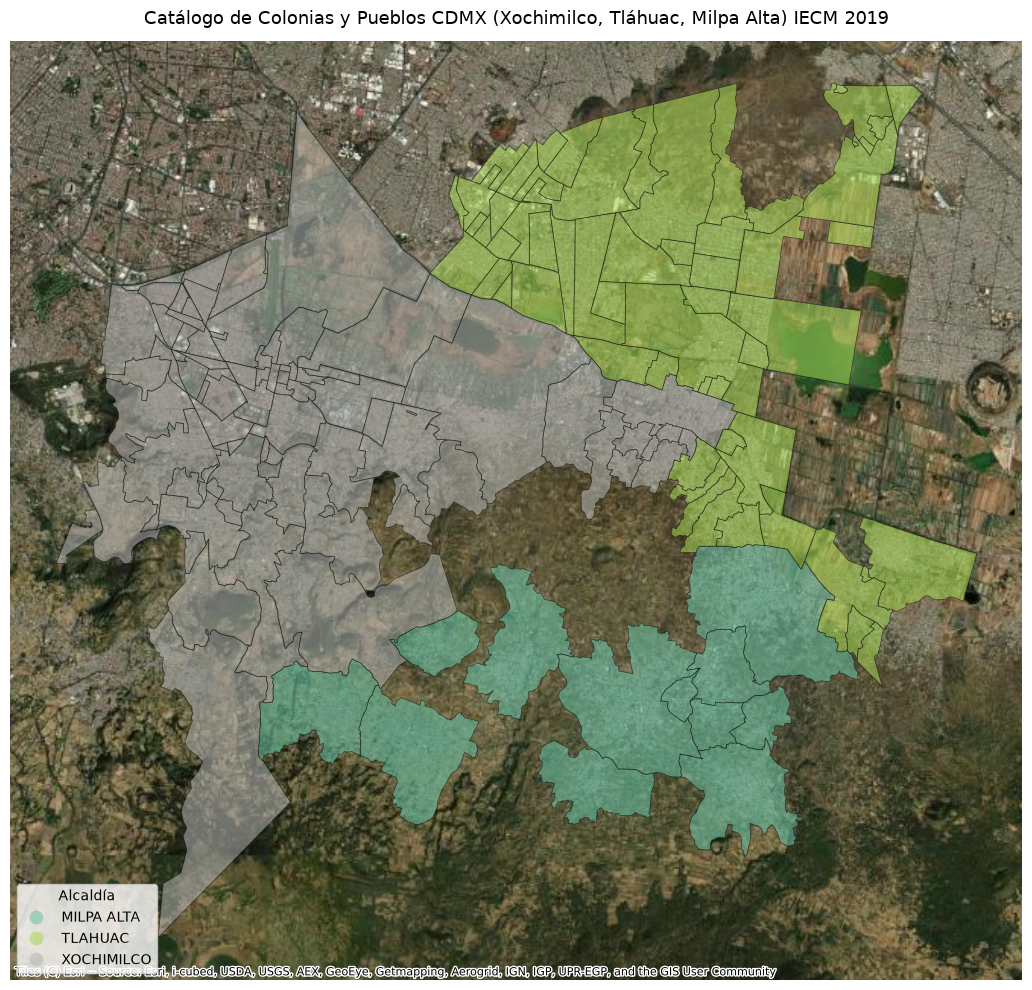
\includegraphics[keepaspectratio]{exploracion_files/figure-pdf/cell-6-output-1.png}}

\subsection{Delimitación territorial}\label{delimitaciuxf3n-territorial}

La alcaldía Xochimilco (\citeproc{ref-xocBarrios}{2026})

\protect\phantomsection\label{refs}
\begin{CSLReferences}{1}{1}
\bibitem[\citeproctext]{ref-inegiGlosario}
Estadística y Geografía (INEGI), Instituto Nacional de. s.~f.
\emph{{G}losario --- inegi.org.mx}.
\href{https://www.inegi.org.mx/app/glosario/default.html?p=ENAMIN2008}{Https://www.inegi.org.mx/app/glosario/default.html?p=ENAMIN2008}.

\bibitem[\citeproctext]{ref-xocBarrios}
\emph{{P}{U}{E}{B}{L}{O}{S} {Y} {B}{A}{R}{R}{I}{O}{S} ---
xochimilco.cdmx.gob.mx}. 2026.
\href{https://www.xochimilco.cdmx.gob.mx/pueblos-y-barrios/}{Https://www.xochimilco.cdmx.gob.mx/pueblos-y-barrios/}.

\end{CSLReferences}




\end{document}
